\documentclass{boi2014-se}

\usepackage{enumitem}

\renewcommand{\DayNum}{2}
\renewcommand{\TaskCode}{postmen}
\renewcommand{\TaskName}{Pensionärspost}
\renewcommand{\TaskVersion}{1.1}

\begin{document}
    \begin{wrapfigure}[8]{r}{4cm}
        \vspace{-18pt}
		\includegraphics[width=4cm]{\TaskCode.jpeg}
	\end{wrapfigure}
    Det är år 2036 och Europa är fullt med pensionärer. För att hålla dem
    hälsosamma så har Europas myndighet för majoritetsgrupper (ja, pensionärer
    är en majoritet) tagit fram förslaget att låta dem hantera leveransen
    av den lilla mängd post som fortfarande skickas - oftast till andra pensionärer.

    Myndigheten har tagit fram ett "pensionärspostssystem" som ser ut på följande
    sätt:
    Europa har delats upp i postdistrikt. Varje distrikt har ett gatunätverk bestående
    av gator och korsningar, och det är alltid möjligt att gå längs gator i båda riktningarna.
    I varje distrikt finns det godtyckligt många pensionärer som kan jobba som
    brevbärare. Varje morgon får brevbärarna varsin säck med post som ska levereras
    på en postrunda som täcker en del av gatunätverket. Varje postrunda måste vara
    pensionärskompatibel, vilket innebär att den måste uppfylla följande krav:

    \begin{itemize}
        \item Den börjar och slutar vid samma korsning.
        \item Den passerar aldrig samma korsning mer än en gång. (Pensionärerna får
        ej bli förvirrade).
        \item Den får inte ha en gata gemensam med någon annan postrunda. På så sätt
        försäkras att varje gata kommer att få post utdelad av högst en brevbärare.
    \end{itemize}

    Tillsammans ska postrundorna täcka hela det givna nätverket: varje gata måste
    vara del av precis en postrunda.    

    \Task
    Myndigheten behöver nu mjukvara som, givet en beskrivning av ett postdistrikts 
    gatunätverk, tar fram en uppsättning pensionärskompatibla postrundor som
    täcker hela nätverket.

    \Input
    Indata beskriver ett gatunätverk.

    Den första raden består av två heltal $N$ och $M$. $N$ är antalet korsningar
    i nätverket, och $M$ är antalet gator. Korsningar är indexerade från $1$ till $N$. 

    Var och en av de följande $M$ raderna består av två heltal $u$ och $v$ ($1 \le u, v \le N, u \neq v$),
    som beskriver att det finns en gata mellan korsningarna $u$ och $v$.

    För all indata gäller:
    \begin{enumerate}
        \item Ett par av korsningar kan inte vara sammankopplade med mer än en gata.
        \item Nätverket är sammanhängande, d.v.s. det är möjligt att ta sig mellan vilka två korsningar som helst genom att förflytta sig längs gatorna.
        \item Det finns en lösning, d.v.s. en mängd pensionärskompatibla postrundor som täcker hela nätverket.
    \end{enumerate}

    \Output
    Varje rad i utdata ska beskriva en pensionärskompatibel postrunda genom
    att ange index för de korsningar som ingår i rundan, i ordningen som de
    besöks. Korsningen som postrundan börjar och slutar på ska bara skrivas ut
    en gång.

    Om det finns mer än en lösning så kan ditt program skriva ut vilken
    som helst av dem.

    \Example

    \example
    {
        10 15 \newline
        1 2 \newline
        5 1\newline
        2 3 \newline
        9 2\newline
        3 4 \newline
        6 3\newline
        4 5 \newline
        7 4\newline
        4 8 \newline
        5 7 \newline
        8 5\newline
        6 7 \newline
        7 8 \newline
        8 10 \newline
        10 9
    }
    {
        2 3 4 5 8 10 9 \newline
        7 8 4 \newline
        1 5 7 6 3
    }
    {
        Följande bild illustrerar gatunätverket och de tre pensionärskompatibla
        postrundor som kan användas för att täcka det.

        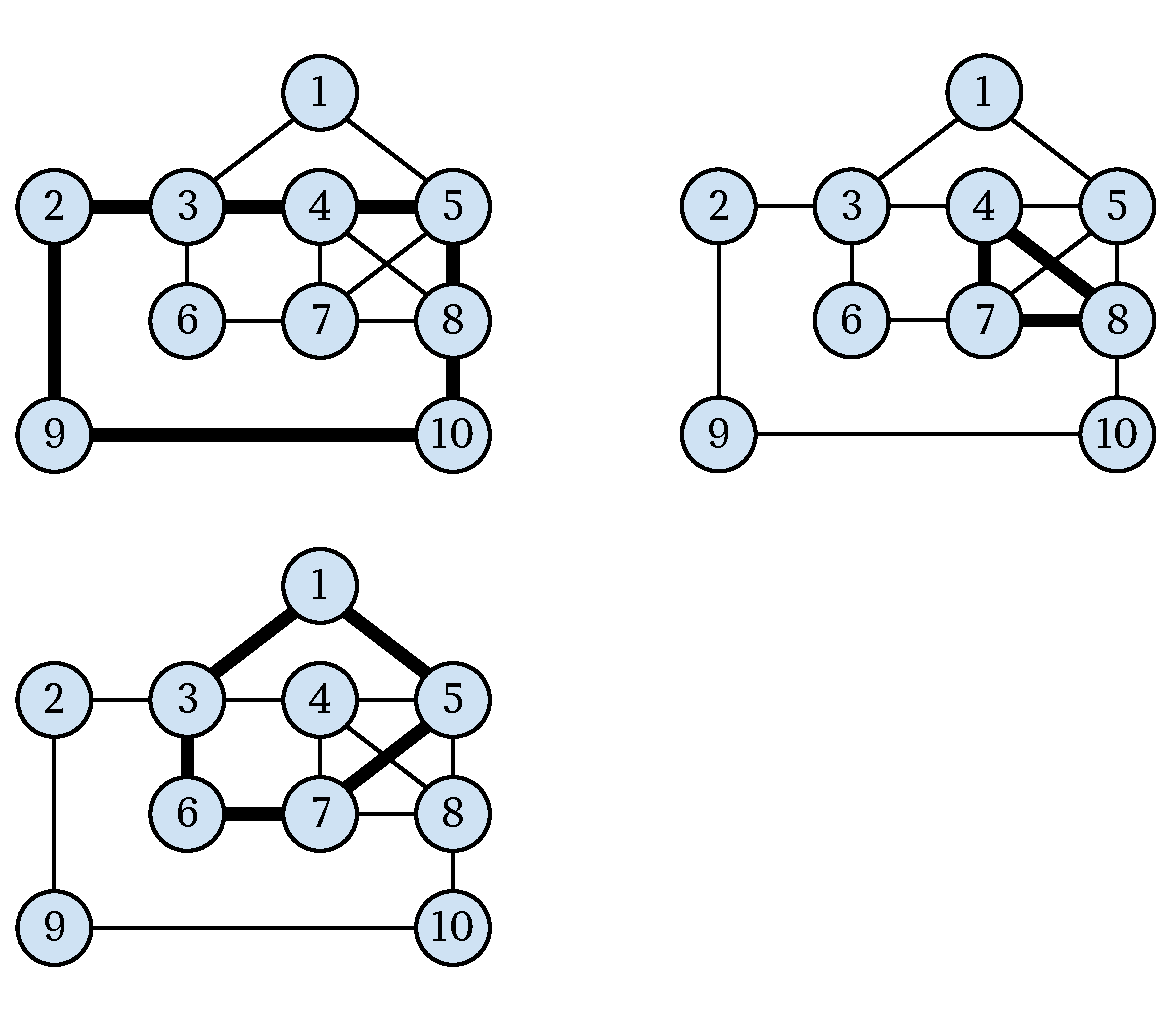
\includegraphics[width=7cm]{senior-example}

        Notera att det finns många lösningar till det här exemplet, även några
        som bara använder två postrundor.
    
    }

    \Scoring

    \begin{description}
        \item[Deluppgift 1 (38 poäng):] $3 \le N \le 2\ 000$, $3 \le M \le 100\ 000$.
        \item[Deluppgift 2 (17 poäng):] $3 \le N \le 100\ 000$, $3 \le M \le 100\ 000$.
        \item[Deluppgift 3 (45 poäng):] $3 \le N \le 500\ 000$, $3 \le M \le 500\ 000$.
    \end{description}

    \Constraints

    \begin{description}
        \item[Tidsgräns:] 0.5 s.
        \item[Minnesgräns:] 256 MB.
    \end{description}

\end{document}
